\documentclass[11pt,a4paper]{scrartcl}
\usepackage{amssymb}
\usepackage{amsmath}
\usepackage{tikz}
\usetikzlibrary{angles,quotes,calc,decorations.markings,intersections}
\input{"../../../../9_klase/1. Vienanariai ir daugianariai/manostilius_lt.sty"}
\title{Geometrija I: įbrėžtinių keturkampų požymiai}
\author{Andrius Berniukevičius}
\begin{document}
\setlength{\parskip}{0.25\baselineskip}
\setlist{nosep}
\setlength{\abovedisplayskip}{8pt plus 2pt minus 2pt}
\setlength{\belowdisplayskip}{8pt plus 2pt minus 2pt}
\maketitle
\section{Įbrėžtiniai keturkampiai}
Keturkampis vadinamas \vocab{įbrėžtiniu}, jei visas jo viršūnes galima išdėstyti ant vieno apskritimo. Tokia sąlyga sieja keturias figūros viršūnes bendru apskritimu ir leidžia taikyti įbrėžtinių kampų savybes: pavyzdžiui, kampai, besiremiantys į tą pačią stygą, yra lygūs, o įbrėžtinio keturkampio priešingų kampų suma lygi $180^\circ$.

Olimpiadinėje geometrijoje šios savybės ypač naudingos sprendžiant kampų radimo uždavinius. Brėžinyje apskritimas ne visada būna duotas iš karto, tačiau kartais jį galime atpažinti arba įrodyti, kad tam tikri keturi taškai priklauso vienam apskritimui. Tuomet atsiveria papildomi ryšiai tarp kampų – tarsi atsirastų tiltas, leidžiantis susieti skirtingose brėžinio vietose esančias figūras. Toliau aptarsime pagrindinius įbrėžtinio keturkampio požymius ir tai, kaip juos pritaikyti kampų medžioklėje.
% ==========================================
% BAZINIAI GINKLAI
% ==========================================
\section{įbrėžtinio keturkampio požymiai}
Kokie požymiai leidžia nustatyti, ar keturkampis yra įbrėžtinis? Toliau aptarsime tris klasikinius požymius. Nustačius, kad tenkinamas bent vienas iš jų, galime pagrįstai teigti, jog keturios keturkampio viršūnės priklauso vienam apskritimui.
\subsection{Priešingų kampų suma}
\begin{proposition}[Įbrėžtinio keturkampio požymis I]
Jei keturkampio priešingų kampų suma lygi $180^\circ$, tai jis yra įbrėžtinis (aplink jį galima apibrėžti apskritimą).
\end{proposition}
\begin{proof}
Ankstesniame handoute aptarėme įbrėžtinio keturkampio savybę: jo priešingų kampų suma lygi $180^\circ$. Dabar įrodysime atvirkštinį teiginį – jei keturkampio priešingų kampų suma lygi $180^\circ$, tai keturkampis yra įbrėžtinis. Įrodymui taikysime prieštaros metodą ir pasinaudosime įgaubto keturkampio kampų savybe, nagrinėta ankstesniame handoute.

\textbf{1 žingsnis.} Tarkime, kad keturkampio $ABCD$ priešingi kampai tenkina sąlygą $\angle A + \angle C = 180^\circ$. Per tris vienoje tiesėje negulinčius taškus $A$, $B$ ir $D$ galima apibrėžti vienintelį apskritimą. Darykime prielaidą, kad taškas $C$ šiam apskritimui nepriklauso ir yra jo viduje.
\begin{center}
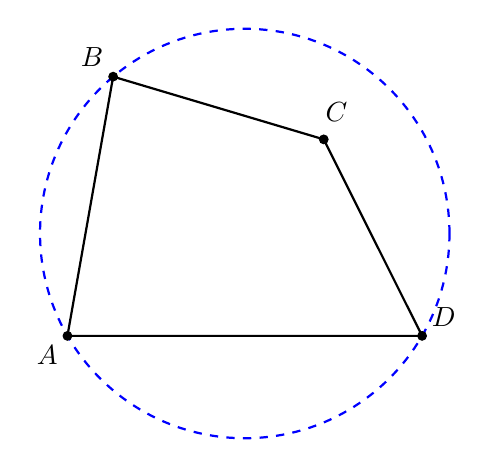
\begin{tikzpicture}[scale=1.3]
    \coordinate (O) at (0,0);
    \draw[thick, dashed, blue] (O) circle (2);
    \coordinate (A) at (210:2);
    \coordinate (B) at (130:2);
    \coordinate (D) at (330:2);
    \coordinate (C_prime) at (50:2); 
    % Taškas C apskritimo viduje
    \coordinate (C) at ($(O)!0.6!(C_prime)$);
    \draw[thick] (A) -- (B) -- (C) -- (D) -- cycle;
    \foreach \p in {A,B,C,D} {\filldraw (\p) circle (1.2pt);}
    \node[below left] at (A) {$A$};
    \node[above left] at (B) {$B$};
    \node[above right, xshift=-1mm, yshift=1mm] at (C) {$C$};
    \node[above right] at (D) {$D$};
\end{tikzpicture}
\end{center}
\textbf{2 žingsnis.} Pažymėkime tašką $C'$ tame lanke $BD$, kuriame nėra taško $A$, taip, kad $C$ būtų trikampio $\triangle BC'D$ viduje. Taškai $A$, $B$, $C'$ ir $D$ priklauso tam pačiam apskritimui, todėl keturkampis $ABC'D$ yra įbrėžtinis.
\begin{center}
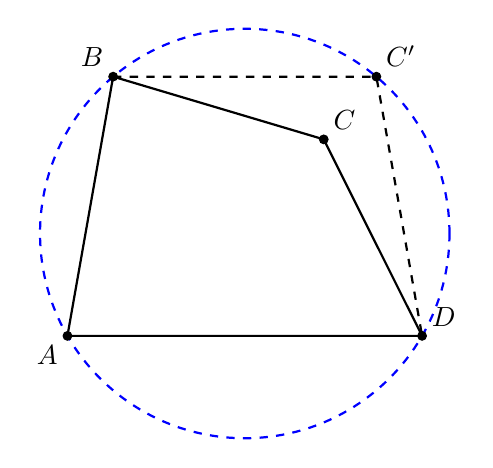
\begin{tikzpicture}[scale=1.3]
    \coordinate (O) at (0,0);
    \draw[thick, dashed, blue] (O) circle (2);
    \coordinate (A) at (210:2);
    \coordinate (B) at (130:2);
    \coordinate (D) at (330:2);
    \coordinate (C_prime) at (50:2); 
    \coordinate (C) at ($(O)!0.6!(C_prime)$);
    \draw[thick] (A) -- (B) -- (C) -- (D) -- cycle;
    \draw[thick, dashed] (B) -- (C_prime) -- (D);
    \foreach \p in {A,B,C,D,C_prime} {\filldraw (\p) circle (1.2pt);}
    \node[below left] at (A) {$A$};
    \node[above left] at (B) {$B$};
    \node[above right] at (C) {$C$};
    \node[above right] at (D) {$D$};
    \node[above right] at (C_prime) {$C'$};
\end{tikzpicture}
\end{center}
\textbf{3 žingsnis.} Kadangi keturkampis $ABC'D$ yra įbrėžtinis, jo priešingų kampų suma lygi $180^\circ$:
\begin{equation*}
\angle A + \angle C' = 180^\circ \implies \angle C' = 180^\circ - \angle A
\end{equation*}
Tačiau pagal mūsų pradinę sąlygą $\angle A + \angle C = 180^\circ$, todėl $\angle C = 180^\circ - \angle A$.
Vadinasi, kampai prie viršūnių $C$ ir $C'$ privalo būti lygūs: $\angle C = \angle C'$.
\begin{center}
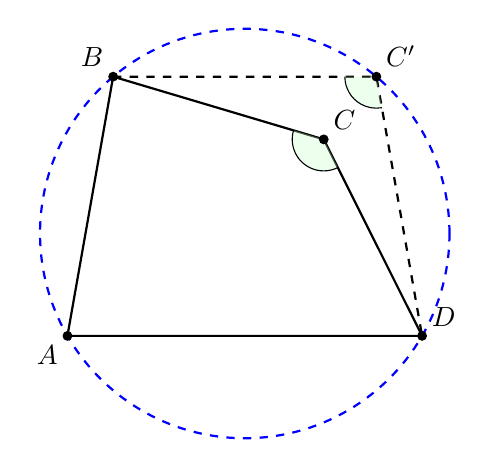
\begin{tikzpicture}[scale=1.3]
    \coordinate (O) at (0,0);
    \draw[thick, dashed, blue] (O) circle (2);
    \coordinate (A) at (210:2);
    \coordinate (B) at (130:2);
    \coordinate (D) at (330:2);
    \coordinate (C_prime) at (50:2); 
    \coordinate (C) at ($(O)!0.6!(C_prime)$);
    \draw[thick] (A) -- (B) -- (C) -- (D) -- cycle;
    \draw[thick, dashed] (B) -- (C_prime) -- (D);
    \pic [draw, fill=green!20, fill opacity=0.35, angle radius=4mm] {angle = B--C_prime--D};
    \pic [draw, fill=green!20, fill opacity=0.35, angle radius=4mm] {angle = B--C--D};
    \foreach \p in {A,B,C,D,C_prime} {\filldraw (\p) circle (1.2pt);}
    \node[below left] at (A) {$A$};
    \node[above left] at (B) {$B$};
    \node[above right] at (C) {$C$};
    \node[above right] at (D) {$D$};
    \node[above right] at (C_prime) {$C'$};
\end{tikzpicture}
\end{center}
\textbf{4 žingsnis.} Taškai $B$, $C'$, $D$ ir $C$ sudaro įgaubtą keturkampį („bumerangą“). Įgaubtosios viršūnės priekampis lygus kitų trijų vidaus kampų sumai:
\begin{equation*}
\angle BCD = \angle BC'D + \angle C'BC + \angle C'DC
\end{equation*}
Vadinasi, $\angle BCD$ yra griežtai didesnis už $\angle BC'D$, nes prie $\angle BC'D$ pridedami du teigiami kampai. Tačiau 3-iajame žingsnyje nustatėme, kad šie kampai lygūs. Gauta prieštara paneigia prielaidą, kad $C$ yra apskritimo viduje. Analogiškai atmetama ir galimybė, kad $C$ yra apskritimo išorėje. Taigi $C$ priklauso apskritimui, einančiam per $A$, $B$ ir $D$, todėl keturkampis $ABCD$ yra įbrėžtinis.
\end{proof}
\subsection{Vienodų įbrėžtinių kampų požymis}
\begin{proposition}[Įbrėžtinio keturkampio požymis II]
Jei taškai $A$ ir $D$ yra toje pačioje tiesės $BC$ pusėje ir $\angle BAC=\angle BDC$, tai taškai $A$, $B$, $C$ ir $D$ priklauso vienam apskritimui.
\end{proposition}
\begin{proof}
Įbrėžtiniai kampai, besiremiantys į tą pačią stygą, yra lygūs. Dabar įrodysime atvirkštinį teiginį: jei $\angle BAC=\angle BDC$, o taškai $A$ ir $D$ yra toje pačioje tiesės $BC$ pusėje, tai keturi taškai $A$, $B$, $C$ ir $D$ yra viename apskritime. Taikysime prieštaros metodą.

\textbf{1 žingsnis.} Pažymėkime taškus $A$, $B$, $C$ ir $D$ taip, kad $A$ ir $D$ būtų toje pačioje tiesės $BC$ pusėje ir $\angle BAC=\angle BDC=\alpha$. Šiame brėžinyje pavaizduojame tik sąlygoje nurodytus taškus ir atkarpas.
\begin{center}
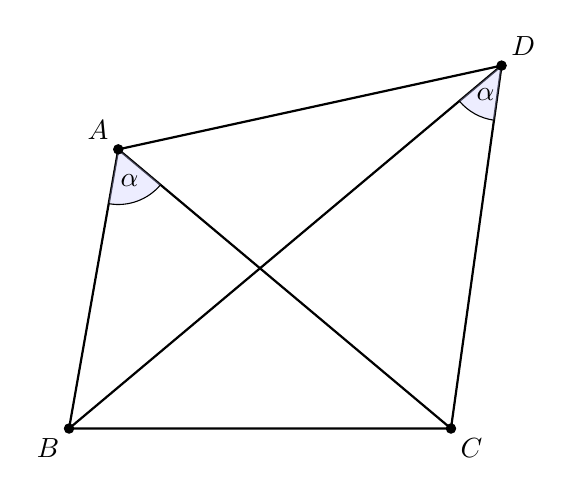
\begin{tikzpicture}[scale=1.4]
    \coordinate (A) at (130:2);
    \coordinate (B) at (210:2);
    \coordinate (C) at (330:2);
    \coordinate (D_prime) at (50:2);
    \coordinate (D) at ($(B)!1.3!(D_prime)$);
    \draw[thick] (A) -- (B) -- (C) -- (D) -- cycle;
    \draw[thick] (A) -- (C);
    \draw[thick] (B) -- (D);
    \pic [draw, fill=blue!20, fill opacity=0.35, "$\alpha$", angle radius=7mm, pic text options={text=black,text opacity=1}] {angle = B--A--C};
    \pic [draw, fill=blue!20, fill opacity=0.35, "$\alpha$", angle radius=7mm, pic text options={text=black,text opacity=1}] {angle = B--D--C};
    \foreach \p in {A,B,C,D} {\filldraw (\p) circle (1.2pt);}
    \node[above left] at (A) {$A$};
    \node[below left] at (B) {$B$};
    \node[below right] at (C) {$C$};
    \node[above right] at (D) {$D$};
\end{tikzpicture}
\end{center}
\textbf{2 žingsnis.} Per taškus $A$, $B$ ir $C$ nubrėžkime apskritimą. Tarkime, priešingai, kad taškas $D$ šiam apskritimui nepriklauso. Kadangi $A$ ir $D$ yra toje pačioje tiesės $BC$ pusėje, brėžinyje nagrinėjame atvejį, kai $D$ yra apskritimo išorėje. Kampų $\angle BAC$ ir $\angle BDC$ lygybė išlieka duota sąlyga; prieštaros prielaida tėra taško $D$ nepriklausymas apskritimui.
\begin{center}
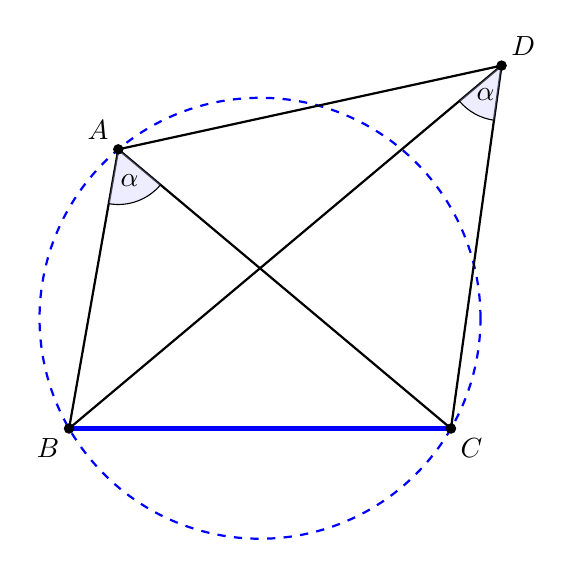
\begin{tikzpicture}[scale=1.4]
    \coordinate (O) at (0,0);
    \draw[thick, dashed, blue] (O) circle (2);
    \coordinate (B) at (210:2);
    \coordinate (C) at (330:2);
    \coordinate (A) at (130:2);
    \coordinate (D_prime) at (50:2);
    \coordinate (D) at ($(B)!1.3!(D_prime)$);
    \draw[thick] (A) -- (B) -- (C) -- (D) -- cycle;
    \draw[thick] (B) -- (D);
    \draw[thick] (A) -- (C);
    \draw[ultra thick, blue] (B) -- (C);
    \pic [draw, fill=blue!20, fill opacity=0.35, "$\alpha$", angle radius=7mm, pic text options={text=black,text opacity=1}] {angle = B--A--C};
    \pic [draw, fill=blue!20, fill opacity=0.35, "$\alpha$", angle radius=7mm, pic text options={text=black,text opacity=1}] {angle = B--D--C};
    \foreach \p in {A,B,C,D} {\filldraw (\p) circle (1.2pt);}
    \node[above left] at (A) {$A$};
    \node[below left] at (B) {$B$};
    \node[below right] at (C) {$C$};
    \node[above right] at (D) {$D$};
\end{tikzpicture}
\end{center}
\textbf{3 žingsnis.} Tiesė $BD$ antrą kartą kerta apskritimą taške $D'$. Sujunkime $C$ su $D'$. Taškai $A$, $B$, $C$ ir $D'$ priklauso tam pačiam apskritimui, todėl kampai, besiremiantys į stygą $BC$, yra lygūs.
\begin{center}
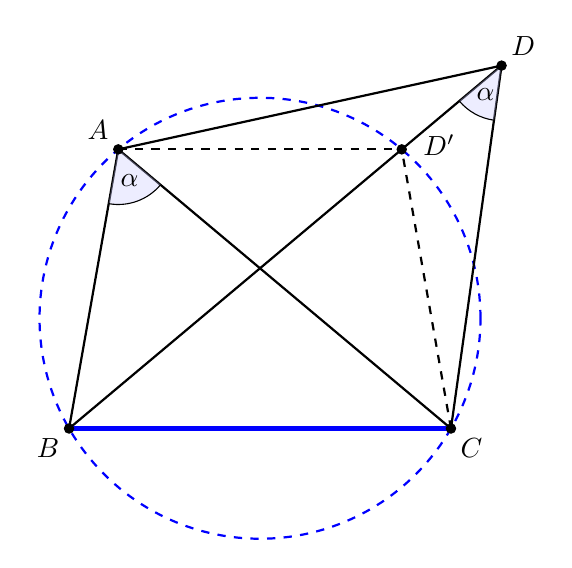
\begin{tikzpicture}[scale=1.4]
    \coordinate (O) at (0,0);
    \draw[thick, dashed, blue] (O) circle (2);
    \coordinate (B) at (210:2);
    \coordinate (C) at (330:2);
    \coordinate (A) at (130:2);
    \coordinate (D_prime) at (50:2);
    \coordinate (D) at ($(B)!1.3!(D_prime)$);
    \draw[thick] (A) -- (B) -- (C) -- (D) -- cycle;
    \draw[thick] (B) -- (D);
    \draw[thick] (A) -- (C);
    \draw[thick, dashed] (C) -- (D_prime);
    \draw[thick, dashed] (A) -- (D_prime);
    \draw[ultra thick, blue] (B) -- (C);
    \pic [draw, fill=blue!20, fill opacity=0.35, "$\alpha$", angle radius=7mm, pic text options={text=black,text opacity=1}] {angle = B--A--C};
    \pic [draw, fill=blue!20, fill opacity=0.35, "$\alpha$", angle radius=7mm, pic text options={text=black,text opacity=1}] {angle = B--D--C};
    \foreach \p in {A,B,C,D,D_prime} {\filldraw (\p) circle (1.2pt);}
    \node[above left] at (A) {$A$}; \node[below left] at (B) {$B$}; \node[below right] at (C) {$C$};
    \node[above right] at (D) {$D$}; \node[above right,xshift = 1.5mm,yshift = -2mm] at (D_prime) {$D'$};
\end{tikzpicture}
\end{center}
\textbf{4 žingsnis.} Kadangi $A$, $B$, $C$ ir $D'$ yra viename apskritime, įbrėžtiniai kampai $\angle BD'C$ ir $\angle BAC$, besiremiantys į tą pačią stygą $BC$, yra lygūs. Iš pradinės sąlygos taip pat žinome, kad $\angle BDC=\angle BAC=\alpha$. Taigi $\angle BD'C=\angle BDC$.
\begin{center}
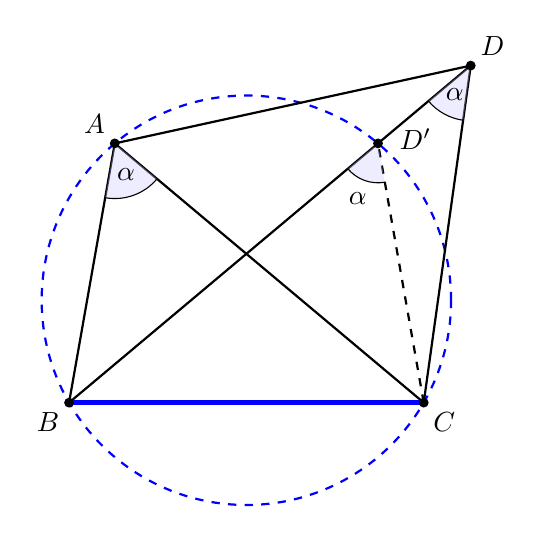
\begin{tikzpicture}[scale=1.3]
    \coordinate (O) at (0,0);
    \draw[thick, dashed, blue] (O) circle (2);
    \coordinate (B) at (210:2); \coordinate (C) at (330:2); \coordinate (A) at (130:2);
    \coordinate (D_prime) at (50:2);
    \coordinate (D) at ($(B)!1.3!(D_prime)$);
    \draw[thick] (A) -- (B) -- (C) -- (D) -- cycle;
    \draw[thick] (B) -- (D); \draw[thick] (A) -- (C);
    \draw[thick, dashed] (C) -- (D_prime);
    \draw[ultra thick, blue] (B) -- (C);
    \pic [draw, fill=blue!20, fill opacity=0.35, "$\alpha$", angle radius=7mm, pic text options={text=black,text opacity=1}] {angle = B--A--C};
    \pic [draw, fill=blue!20, fill opacity=0.35, "$\alpha$", angle radius=7mm, pic text options={text=black,text opacity=1}] {angle = B--D--C};
    \pic [draw, fill=blue!20, fill opacity=0.35, "$\alpha$", angle radius=5mm, angle eccentricity=1.5, pic text options={text=black,text opacity=1}] {angle = B--D_prime--C};
    \foreach \p in {A,B,C,D,D_prime} {\filldraw (\p) circle (1.2pt);}
    \node[above left] at (A) {$A$}; \node[below left] at (B) {$B$}; \node[below right] at (C) {$C$};
    \node[above right] at (D) {$D$}; \node[above right,xshift = 1.5mm,yshift = -2mm] at (D_prime) {$D'$};
\end{tikzpicture}
\end{center}
\textbf{5 žingsnis.} Taškai $C$, $D$ ir $D'$ sudaro trikampį $\triangle CDD'$. Kadangi taškai $B$, $D'$ ir $D$ yra vienoje tiesėje, kampas $\angle BD'C$ yra trikampio $\triangle CDD'$ priekampis ties viršūne $D'$. Pagal trikampio priekampio teoremą:
\begin{equation*}
\angle BD'C = \angle D'DC + \angle D'CD
\end{equation*}
Kadangi $\angle D'CD>0^\circ$, iš lygybės seka griežta nelygybė $\angle BD'C>\angle D'DC$. O spinduliai $DB$ ir $DD'$ sutampa, todėl $\angle D'DC=\angle BDC$. Vadinasi,
\begin{equation*}
\angle BD'C > \angle BDC.
\end{equation*}
Tačiau 4-ajame žingsnyje nustatėme, kad $\angle BD'C=\angle BDC$; gauta prieštara paneigia prielaidą, jog $D$ yra apskritimo išorėje.

Jei $D$ būtų apskritimo viduje, jis būtų tarp $B$ ir antrosios tiesės $BD$ sankirtos su apskritimu $D'$. Tuomet $\angle BDC$ būtų trikampio $\triangle CDD'$ priekampis ties $D$, todėl $\angle BDC>\angle BD'C$. Tai vėl prieštarautų 4-ajame žingsnyje gautai kampų lygybei. Taigi $D$ negali būti nei apskritimo viduje, nei išorėje; vadinasi, jis priklauso apskritimui, einančiam per $A$, $B$ ir $C$.
\end{proof}
\subsection{Priekampio požymis}
\begin{proposition}[Įbrėžtinio keturkampio požymis III]
Jei iškiliojo keturkampio priekampis lygus priešingam vidiniam kampui, tai keturkampis yra įbrėžtinis.
\end{proposition}
\begin{proof}
Šį teiginį gausime iš įbrėžtinio keturkampio požymio pagal priešingų kampų sumą.

\textbf{1 žingsnis.} Nagrinėkime iškilųjį keturkampį $ABCD$ ir pratęskime kraštinę $CD$ už taško $D$ iki taško $E$. Pagal sąlygą priekampis $\angle ADE$ lygus priešingam vidiniam kampui $\angle ABC$. Pažymėkime šių kampų bendrąjį didumą $\beta$.
\begin{center}
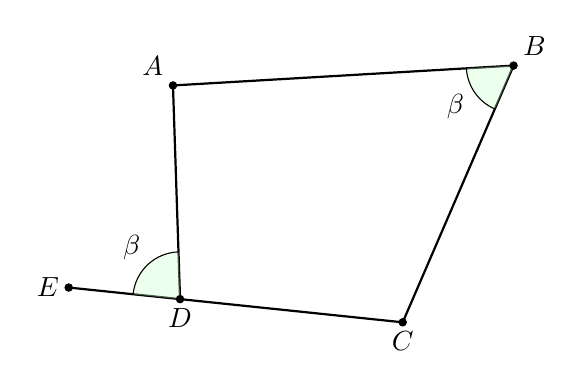
\begin{tikzpicture}[scale=1.1]
    \coordinate (A) at (145:2.2);
    \coordinate (B) at (35:2.6);
    \coordinate (C) at (300:1.7);
    \coordinate (D) at (215:2.1);
    \coordinate (E) at ($(C)!1.5!(D)$);
    \draw[thick] (A) -- (B) -- (C) -- (D) -- cycle;
    \draw[thick] (D) -- (E);
    \pic [draw, fill=green!20, fill opacity=0.35, "$\beta$", angle radius=6mm, angle eccentricity=1.5, pic text options={text=black,text opacity=1}] {angle = A--B--C};
    \pic [draw, fill=green!20, fill opacity=0.35, "$\beta$", angle radius=6mm, angle eccentricity=1.5, pic text options={text=black,text opacity=1}] {angle = A--D--E};
    \foreach \p in {A,B,C,D,E} {\filldraw (\p) circle (1.2pt);}
    \node[above left] at (A) {$A$}; \node[above right] at (B) {$B$};
    \node[below] at (C) {$C$}; \node[below] at (D) {$D$};
    \node[left] at (E) {$E$};
\end{tikzpicture}
\end{center}
\textbf{2 žingsnis.} Kadangi spinduliai $DC$ ir $DE$ yra priešingi, kampai $\angle ADC$ ir $\angle ADE$ yra gretutiniai. Todėl
\begin{equation*} 
\angle ADC = 180^\circ - \angle ADE = 180^\circ - \beta
\end{equation*}
\begin{center}
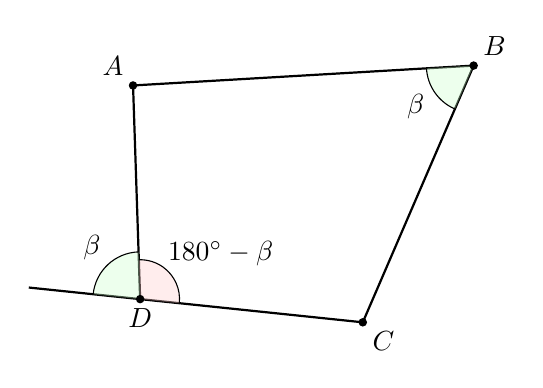
\begin{tikzpicture}[scale=1.1]
    \coordinate (A) at (145:2.2);
    \coordinate (B) at (35:2.6);
    \coordinate (C) at (300:1.7);
    \coordinate (D) at (215:2.1);
    \coordinate (E) at ($(C)!1.5!(D)$);
    \draw[thick] (A) -- (B) -- (C) -- (D) -- cycle;
    \draw[thick] (D) -- (E);
    \pic [draw, fill=green!20, fill opacity=0.35, "$\beta$", angle radius=6mm, angle eccentricity=1.5, pic text options={text=black,text opacity=1}] {angle = A--B--C};
    \pic [draw, fill=green!20, fill opacity=0.35, "$\beta$", angle radius=6mm, angle eccentricity=1.5, pic text options={text=black,text opacity=1}] {angle = A--D--E};
    \pic [draw, fill=red!20, fill opacity=0.35, "$180^\circ-\beta$", angle radius=5mm, angle eccentricity=1.7, pic text options={text=black,text opacity=1, xshift=4mm}] {angle = C--D--A};
    \foreach \p in {A,B,C,D} {\filldraw (\p) circle (1.2pt);}
    \node[above left] at (A) {$A$}; \node[above right] at (B) {$B$};
    \node[below right] at (C) {$C$}; \node[below] at (D) {$D$};
\end{tikzpicture}
\end{center}
\textbf{3 žingsnis.} Apskaičiuokime keturkampio $ABCD$ priešingų vidinių kampų $\angle ABC$ ir $\angle ADC$ sumą:
\begin{equation*}
\angle B + \angle ADC = \beta + (180^\circ - \beta) = 180^\circ
\end{equation*}
Kadangi priešingų kampų suma lygi $180^\circ$, pagal I įbrėžtinio keturkampio požymį keturkampis $ABCD$ yra įbrėžtinis.
\begin{center}
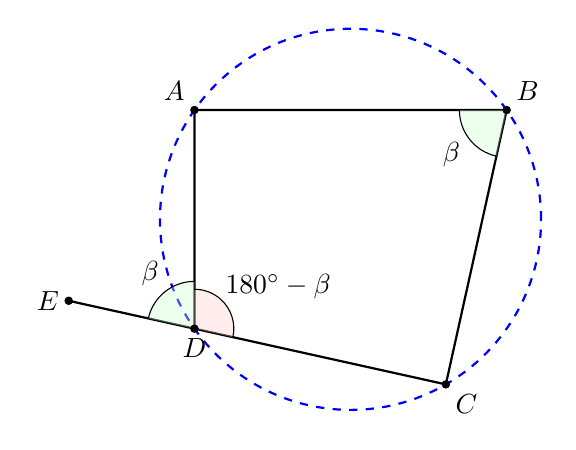
\begin{tikzpicture}[scale=1.1]
    \coordinate (A) at (145:2.2);
    \coordinate (B) at (35:2.2);
    \coordinate (C) at (300:2.2);
    \coordinate (D) at (215:2.2);
    \coordinate (E) at ($(C)!1.5!(D)$);
    \draw[thick, dashed, blue] (0,0) circle (2.2);
    \draw[thick] (A) -- (B) -- (C) -- (D) -- cycle;
    \draw[thick] (D) -- (E);
    \pic [draw, fill=green!20, fill opacity=0.35, "$\beta$", angle radius=6mm, angle eccentricity=1.5, pic text options={text=black,text opacity=1}] {angle = A--B--C};
    \pic [draw, fill=green!20, fill opacity=0.35, "$\beta$", angle radius=6mm, angle eccentricity=1.5, pic text options={text=black,text opacity=1}] {angle = A--D--E};
    \pic [draw, fill=red!20, fill opacity=0.35, "$180^\circ-\beta$", angle radius=5mm, angle eccentricity=1.7, pic text options={text=black,text opacity=1, xshift=4mm}] {angle = C--D--A};
    \foreach \p in {A,B,C,D,E} {\filldraw (\p) circle (1.2pt);}
    \node[above left] at (A) {$A$};
    \node[above right] at (B) {$B$};
    \node[below right] at (C) {$C$};
    \node[below] at (D) {$D$};
    \node[left] at (E) {$E$};
\end{tikzpicture}
\end{center}
\end{proof}
% ==========================================
% PAVYZDŽIAI
% ==========================================
\section{Aukštinių konfigūracija ir įbrėžtiniai keturkampiai}
Panagrinėkime dažnai olimpiadinėje geometrijoje pasitaikančią konfigūraciją, kurioje aukštinių statmenumas leidžia nustatyti kelis įbrėžtinius keturkampius. Šių keturkampių savybės padeda susieti skirtingose brėžinio vietose esančius kampus.
\begin{example}[Aukštinių pagrindų nulemti įbrėžtiniai keturkampiai]
Smailiajame trikampyje $\triangle ABC$ nubrėžtos aukštinės $BD$ ir $CE$, kurios susikerta taške $H$. Įrodykite, kad:
\begin{enumerate}
    \renewcommand{\labelenumi}{\arabic{enumi})}
    \item Keturkampis $BCDE$ yra įbrėžtinis.
    \item Keturkampis $ADHE$ yra įbrėžtinis.
    \item $\angle DAH = \angle DBC$.
\end{enumerate}
\end{example}
\begin{proof}
Įrodyme pasitelksime aukštinių statmenumo savybę ir įbrėžtinio keturkampio požymius.

\textbf{1 žingsnis.} Nubrėžkime smailųjį trikampį $\triangle ABC$ ir aukštines $BD \perp AC$ bei $CE \perp AB$. Jų susikirtimo tašką pažymėkime $H$. Pažymėkime brėžinyje aukštinių ir trikampio kraštinių sudaromus stačiuosius kampus.
\begin{center}
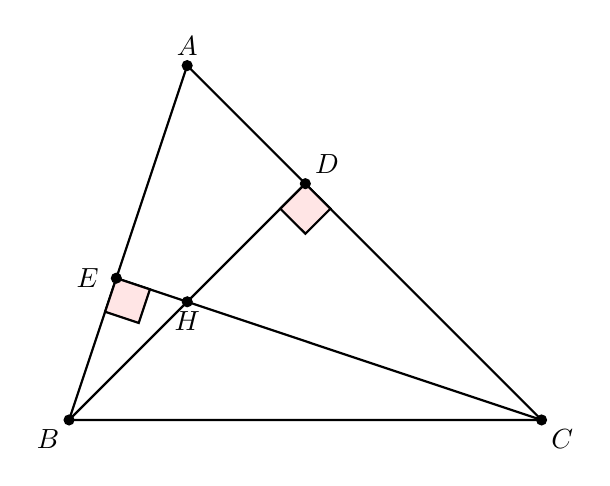
\begin{tikzpicture}[scale=1.5]
    \coordinate (A) at (1,3);
    \coordinate (B) at (0,0);
    \coordinate (C) at (4,0);
    \coordinate (D) at ($(A)!(B)!(C)$);
    \coordinate (E) at ($(A)!(C)!(B)$);
    \coordinate (H) at (intersection of B--D and C--E);
    \draw[thick] (A) -- (B) -- (C) -- cycle;
    \draw[thick] (B) -- (D);
    \draw[thick] (C) -- (E);
    \coordinate (dirC_D) at ($(D)!3mm!(C)$);
    \coordinate (dirB_D) at ($(D)!3mm!(B)$);
    \coordinate (rect_D) at ($(dirC_D) + (dirB_D) - (D)$);
    \draw[thick, fill=red!10] (dirC_D) -- (rect_D) -- (dirB_D) -- (D) -- cycle;
    \coordinate (dirB_E) at ($(E)!3mm!(B)$);
    \coordinate (dirC_E) at ($(E)!3mm!(C)$);
    \coordinate (rect_E) at ($(dirB_E) + (dirC_E) - (E)$);
    \draw[thick, fill=red!10] (dirB_E) -- (rect_E) -- (dirC_E) -- (E) -- cycle;
    \foreach \p in {A,B,C,D,E,H} {\filldraw (\p) circle (1.2pt);}
    \node[above] at (A) {$A$}; \node[below left] at (B) {$B$}; \node[below right] at (C) {$C$};
    \node[above right] at (D) {$D$}; \node[left, xshift=-1mm] at (E) {$E$}; \node[below] at (H) {$H$};
\end{tikzpicture}
\end{center}
\textbf{2 žingsnis.} Nagrinėkime keturkampį $BCDE$. Kadangi $BD \perp AC$ ir $D \in AC$, tai $\angle BDC=90^\circ$. Taip pat $CE \perp AB$ ir $E \in AB$, todėl $\angle BEC=90^\circ$. Taigi $\angle BDC=\angle BEC$. Be to, taškai $D$ ir $E$ yra toje pačioje tiesės $BC$ pusėje. Vadinasi, pagal vienodų įbrėžtinių kampų požymį keturkampis $BCDE$ yra įbrėžtinis.
Nubrėžkime šį keturkampį apibrėžiantį apskritimą.
\begin{equation*} 
\angle BEC = \angle BDC = 90^\circ \implies BCDE \text{ – įbrėžtinis}
\end{equation*}
\begin{center}
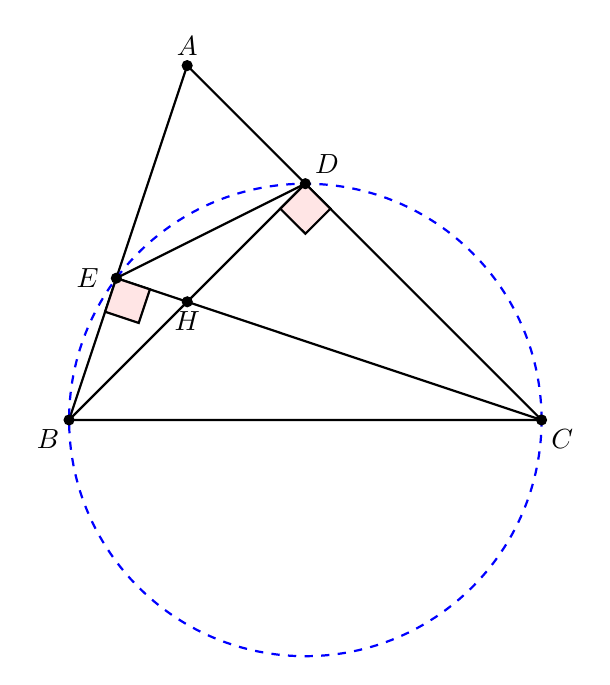
\begin{tikzpicture}[scale=1.5]
    \coordinate (A) at (1,3);
    \coordinate (B) at (0,0);
    \coordinate (C) at (4,0);
    \coordinate (D) at ($(A)!(B)!(C)$);
    \coordinate (E) at ($(A)!(C)!(B)$);
    \coordinate (H) at (intersection of B--D and C--E);
    \draw[thick] (A) -- (B) -- (C) -- cycle;
    \draw[thick] (B) -- (D);
    \draw[thick] (C) -- (E);
    \coordinate (M) at ($(B)!0.5!(C)$);
    \draw[thick, dashed, blue] (M) circle (2);
    \coordinate (dirC_D) at ($(D)!3mm!(C)$); \coordinate (dirB_D) at ($(D)!3mm!(B)$); \coordinate (rect_D) at ($(dirC_D)+(dirB_D)-(D)$);
    \draw[thick, fill=red!10] (dirC_D)--(rect_D)--(dirB_D)--(D)--cycle;
    \coordinate (dirB_E) at ($(E)!3mm!(B)$); \coordinate (dirC_E) at ($(E)!3mm!(C)$); \coordinate (rect_E) at ($(dirB_E)+(dirC_E)-(E)$);
    \draw[thick, fill=red!10] (dirB_E)--(rect_E)--(dirC_E)--(E)--cycle;
    \draw[thick] (E) -- (D);
    \foreach \p in {A,B,C,D,E,H} {\filldraw (\p) circle (1.2pt);}
    \node[above] at (A) {$A$}; \node[below left] at (B) {$B$}; \node[below right] at (C) {$C$};
    \node[above right] at (D) {$D$}; \node[left, xshift=-1mm] at (E) {$E$}; \node[below] at (H) {$H$};
\end{tikzpicture}
\end{center}
\textbf{3 žingsnis.} Dabar nagrinėkime keturkampį $ADHE$. Jo priešingi kampai ties $D$ ir $E$ yra statieji, todėl jų suma lygi:
\begin{equation*} 
\angle AEH + \angle ADH = 90^\circ + 90^\circ = 180^\circ 
\end{equation*}
Kadangi keturkampio $ADHE$ priešingų kampų suma lygi $180^\circ$, pagal priešingų kampų sumos požymį jis yra įbrėžtinis. Nubrėžkime apie jį apskritimą (brėžinyje – raudona punktyrinė linija) ir atkarpą $AH$.
\begin{center}
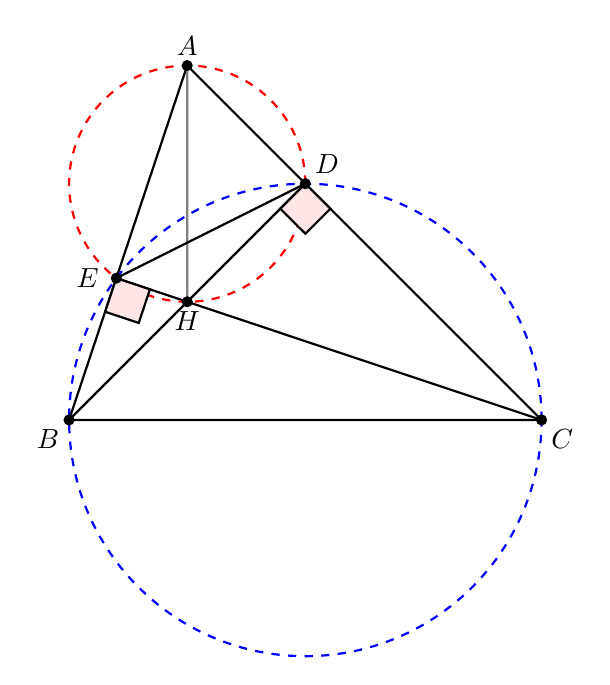
\begin{tikzpicture}[scale=1.5]
    \coordinate (A) at (1,3);
    \coordinate (B) at (0,0);
    \coordinate (C) at (4,0);
    \coordinate (D) at ($(A)!(B)!(C)$);
    \coordinate (E) at ($(A)!(C)!(B)$);
    \coordinate (H) at (intersection of B--D and C--E);
    \draw[thick] (A) -- (B) -- (C) -- cycle;
    \draw[thick] (B) -- (D);
    \draw[thick] (C) -- (E);
    \draw[thick, gray] (A) -- (H);
    \coordinate (M1) at ($(B)!0.5!(C)$);
    \draw[thick, dashed, blue] (M1) circle (2);
    \coordinate (M2) at ($(A)!0.5!(H)$);
    \draw[thick, dashed, red] (M2) circle (1);
    \coordinate (dirC_D) at ($(D)!3mm!(C)$); \coordinate (dirB_D) at ($(D)!3mm!(B)$); \coordinate (rect_D) at ($(dirC_D)+(dirB_D)-(D)$);
    \draw[thick, fill=red!10] (dirC_D)--(rect_D)--(dirB_D)--(D)--cycle;
    \coordinate (dirB_E) at ($(E)!3mm!(B)$); \coordinate (dirC_E) at ($(E)!3mm!(C)$); \coordinate (rect_E) at ($(dirB_E)+(dirC_E)-(E)$);
    \draw[thick, fill=red!10] (dirB_E)--(rect_E)--(dirC_E)--(E)--cycle;
    \draw[thick] (E) -- (D);
    \foreach \p in {A,B,C,D,E,H} {\filldraw (\p) circle (1.2pt);}
    \node[above] at (A) {$A$}; \node[below left] at (B) {$B$}; \node[below right] at (C) {$C$};
    \node[above right] at (D) {$D$}; \node[left, xshift=-1mm] at (E) {$E$}; \node[below] at (H) {$H$};
\end{tikzpicture}
\end{center}
\textbf{4 žingsnis.} Pradėkime įrodyti, kad $\angle DAH = \angle DBC$. Kadangi keturkampis $ADHE$ įbrėžtinis, kampai $\angle DAH$ ir $\angle DEH$ remiasi į tą pačią stygą $DH$, todėl jie lygūs.
\begin{equation*}
\angle DAH = \angle DEH
\end{equation*}
\begin{center}
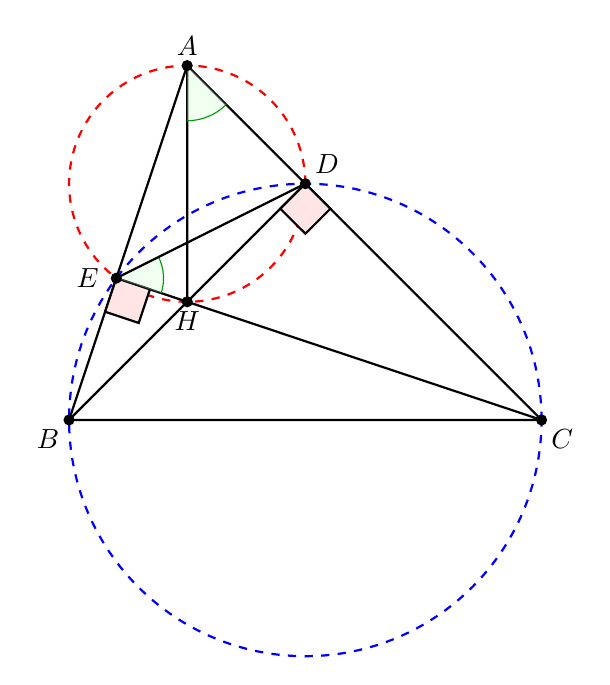
\begin{tikzpicture}[scale=1.5]
    \coordinate (A) at (1,3); \coordinate (B) at (0,0); \coordinate (C) at (4,0);
    \coordinate (D) at ($(A)!(B)!(C)$); \coordinate (E) at ($(A)!(C)!(B)$);
    \coordinate (H) at (intersection of B--D and C--E);
    \draw[thick, dashed, blue] ($(B)!0.5!(C)$) circle (2);
    \draw[thick, dashed, red] ($(A)!0.5!(H)$) circle (1);
    \draw[thick] (A)--(B)--(C)--cycle (B)--(D) (C)--(E) (A)--(H);
    \coordinate (dirC_D) at ($(D)!3mm!(C)$); \coordinate (dirB_D) at ($(D)!3mm!(B)$);
    \coordinate (rect_D) at ($(dirC_D)+(dirB_D)-(D)$);
    \draw[thick, fill=red!10] (dirC_D)--(rect_D)--(dirB_D)--(D)--cycle;
    \coordinate (dirB_E) at ($(E)!3mm!(B)$); \coordinate (dirC_E) at ($(E)!3mm!(C)$);
    \coordinate (rect_E) at ($(dirB_E)+(dirC_E)-(E)$);
    \draw[thick, fill=red!10] (dirB_E)--(rect_E)--(dirC_E)--(E)--cycle;
    \pic [draw=green!60!black, fill=green!20, fill opacity=0.3, angle radius=7mm] {angle = H--A--D};
    \pic [draw=green!60!black, fill=green!20, fill opacity=0.3, angle radius=6mm] {angle = H--E--D};
    % ED piešiame virš stačiųjų kampų žymėjimų, kad atkarpa būtų aiškiai matoma.
    \draw[thick] (E)--(D);
    \foreach \p in {A,B,C,D,E,H} {\filldraw (\p) circle (1.2pt);}
    \node[above] at (A) {$A$}; \node[below left] at (B) {$B$}; \node[below right] at (C) {$C$};
    \node[above right] at (D) {$D$}; \node[left, xshift=-1mm] at (E) {$E$}; \node[below] at (H) {$H$};
\end{tikzpicture}
\end{center}
\textbf{5 žingsnis.} Taškai $E$, $H$ ir $C$ yra vienoje tiesėje, o spinduliai $EH$ ir $EC$ sutampa. Todėl $\angle DEH=\angle DEC$. Kartu su ankstesniame žingsnyje gauta lygybe turime:
\begin{equation*}
\angle DAH = \angle DEH = \angle DEC
\end{equation*}
\textbf{6 žingsnis.} Kadangi keturkampis $BCDE$ įbrėžtinis, kampai $\angle DEC$ ir $\angle DBC$, besiremiantys į tą pačią stygą $DC$, yra lygūs. Taigi gauname:
\begin{equation*}
\angle DAH = \angle DEH = \angle DEC = \angle DBC.
\end{equation*}
\begin{center}
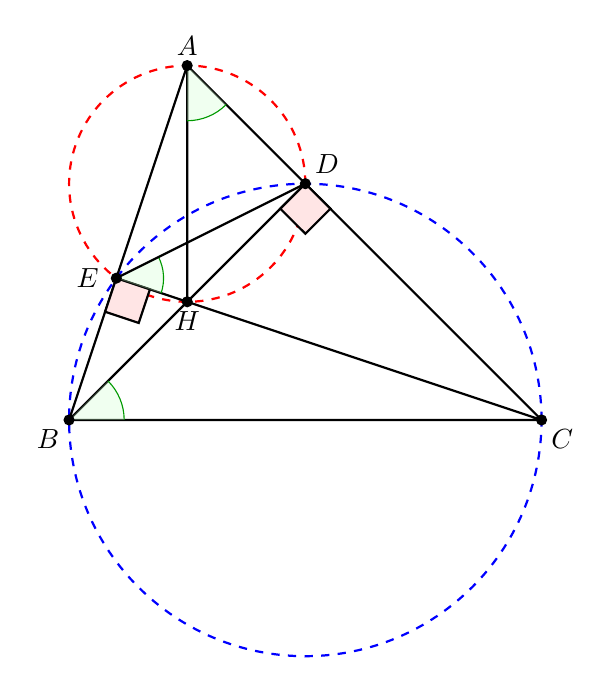
\begin{tikzpicture}[scale=1.5]
    \coordinate (A) at (1,3); \coordinate (B) at (0,0); \coordinate (C) at (4,0);
    \coordinate (D) at ($(A)!(B)!(C)$); \coordinate (E) at ($(A)!(C)!(B)$);
    \coordinate (H) at (intersection of B--D and C--E);
    \draw[thick, dashed, blue] ($(B)!0.5!(C)$) circle (2);
    \draw[thick, dashed, red] ($(A)!0.5!(H)$) circle (1);
    \draw[thick] (A)--(B)--(C)--cycle (B)--(D) (C)--(E) (A)--(H);
    \coordinate (dirC_D) at ($(D)!3mm!(C)$); \coordinate (dirB_D) at ($(D)!3mm!(B)$);
    \coordinate (rect_D) at ($(dirC_D)+(dirB_D)-(D)$);
    \draw[thick, fill=red!10] (dirC_D)--(rect_D)--(dirB_D)--(D)--cycle;
    \coordinate (dirB_E) at ($(E)!3mm!(B)$); \coordinate (dirC_E) at ($(E)!3mm!(C)$);
    \coordinate (rect_E) at ($(dirB_E)+(dirC_E)-(E)$);
    \draw[thick, fill=red!10] (dirB_E)--(rect_E)--(dirC_E)--(E)--cycle;
    \pic [draw=green!60!black, fill=green!20, fill opacity=0.3, angle radius=7mm] {angle = H--A--D};
    \pic [draw=green!60!black, fill=green!20, fill opacity=0.3, angle radius=6mm] {angle = C--E--D};
    \pic [draw=green!60!black, fill=green!20, fill opacity=0.3, angle radius=7mm] {angle = C--B--D};
    \draw[thick] (E)--(D);
    \foreach \p in {A,B,C,D,E,H} {\filldraw (\p) circle (1.2pt);}
    \node[above] at (A) {$A$}; \node[below left] at (B) {$B$}; \node[below right] at (C) {$C$};
    \node[above right] at (D) {$D$}; \node[left, xshift=-1mm] at (E) {$E$}; \node[below] at (H) {$H$};
\end{tikzpicture}
\end{center}
\end{proof}

\begin{example}[Susikertantys apskritimai]
Du apskritimai susikerta taškuose $P$ ir $Q$. Tiesė, einanti per $P$, kerta pirmąjį apskritimą dar taške $A$, o antrąjį – dar taške $B$. Tiesė, einanti per $Q$, kerta pirmąjį apskritimą dar taške $C$, o antrąjį – dar taške $D$. Įrodykite, kad tiesės $AC$ ir $BD$ yra lygiagrečios.
\end{example}

\begin{proof}
\textbf{Sprendimas.} Įbrėžtinių keturkampių savybėmis ir gretutinių kampų ryšiu susiesime kampus, kuriuos kirstinė $AB$ sudaro su tiesėmis $AC$ ir $BD$.

\textbf{1 žingsnis.} Pavaizduokime du apskritimus, jų susikirtimo taškus $P$ ir $Q$, tieses $APB$ ir $CQD$ bei atkarpas $AC$ ir $BD$.
\newcommand{\intersectingCircleFigure}[1]{%
\begin{tikzpicture}[scale=1.3]
    \draw[thick] (-1,0) circle (1.803);
    \draw[thick] (1.5,0) circle (2.121);
    \coordinate (P) at (0,1.5);
    \coordinate (Q) at (0,-1.5);
    \coordinate (A) at (-2.8,0.1);
    \coordinate (B) at (1.2,2.1);
    \coordinate (C) at (-2.5,-1);
    \coordinate (D) at (2.308,-1.962);
    \draw[thick] (A)--(P)--(B);
    \draw[thick] (C)--(Q)--(D);
    \draw[thick] (A)--(C);
    \draw[thick] (B)--(D);
    #1
    \foreach \p/\pos in {P/above,Q/below,A/left,B/above right,C/left,D/right} {
        \fill (\p) circle (1.5pt) node[\pos] {$\p$};
    }
\end{tikzpicture}%
}
\begin{center}
\intersectingCircleFigure{}
\end{center}

\textbf{2 žingsnis.} Nubrėžkime bendrąją stygą $PQ$ ir pažymėkime kampus $\angle CAP$ bei $\angle CQP$. Tarkime, kad $\angle CAP=\alpha$. Keturkampis $ACQP$ yra įbrėžtinis, todėl jo priešingų kampų suma lygi $180^\circ$. Taigi
\begin{equation*}
\angle CQP=180^\circ-\alpha.
\end{equation*}
\begin{center}
\intersectingCircleFigure{%
    \draw[thick,dashed,blue] (P)--(Q);
    \pic[draw=green!60!black,fill=green!20,fill opacity=0.35,angle radius=6mm,pic text={$\alpha$},pic text options={text=black,text opacity=1,font=\bfseries},angle eccentricity=1.4] {angle=C--A--P};
    \pic[draw=red!70!black,fill=red!20,fill opacity=0.35,angle radius=5mm,pic text={$180^\circ-\alpha$},pic text options={text=black,text opacity=1,font=\bfseries,xshift=-3mm},angle eccentricity=1.9] {angle=P--Q--C};
}
\end{center}

\textbf{3 žingsnis.} Taškai $C$, $Q$ ir $D$ yra vienoje tiesėje, todėl kampai $\angle CQP$ ir $\angle PQD$ yra gretutiniai. Vadinasi,
\begin{equation*}
\angle PQD=180^\circ-\angle CQP=\alpha.
\end{equation*}
\begin{center}
\intersectingCircleFigure{%
    \draw[thick,dashed,blue] (P)--(Q);
    \pic[draw=green!60!black,fill=green!20,fill opacity=0.35,angle radius=6mm,pic text={$\alpha$},pic text options={text=black,text opacity=1,font=\bfseries},angle eccentricity=1.4] {angle=C--A--P};
    \pic[draw=red!70!black,fill=red!20,fill opacity=0.35,angle radius=5mm,pic text={$180^\circ-\alpha$},pic text options={text=black,text opacity=1,font=\bfseries,xshift=-3mm},angle eccentricity=1.9] {angle=P--Q--C};
    \pic[draw=green!60!black,fill=green!20,fill opacity=0.35,angle radius=7mm,pic text={$\alpha$},pic text options={text=black,text opacity=1,font=\bfseries},angle eccentricity=1.3] {angle=D--Q--P};
}
\end{center}

\textbf{4 žingsnis.} Keturkampis $PQDB$ yra įbrėžtinis, todėl jo priešingų kampų $\angle PQD$ ir $\angle PBD$ suma lygi $180^\circ$. Todėl
\begin{equation*}
\angle PBD=180^\circ-\angle PQD=180^\circ-\alpha.
\end{equation*}
\begin{center}
\intersectingCircleFigure{%
    \draw[thick,dashed,blue] (P)--(Q);
    \pic[draw=green!60!black,fill=green!20,fill opacity=0.35,angle radius=6mm,pic text={$\alpha$},pic text options={text=black,text opacity=1,font=\bfseries},angle eccentricity=1.4] {angle=C--A--P};
    \pic[draw=red!70!black,fill=red!20,fill opacity=0.35,angle radius=5mm,pic text={$180^\circ-\alpha$},pic text options={text=black,text opacity=1,font=\bfseries,xshift=-3mm},angle eccentricity=1.9] {angle=P--Q--C};
    \pic[draw=green!60!black,fill=green!20,fill opacity=0.35,angle radius=7mm,pic text={$\alpha$},pic text options={text=black,text opacity=1,font=\bfseries},angle eccentricity=1.3] {angle=D--Q--P};
    \pic[draw=red!70!black,fill=red!20,fill opacity=0.35,angle radius=6mm,pic text={$180^\circ-\alpha$},pic text options={text=black,text opacity=1,font=\bfseries},angle eccentricity=1.8] {angle=P--B--D};
}
\end{center}

\textbf{5 žingsnis.} Taškai $A$, $P$ ir $B$ yra vienoje tiesėje, todėl spinduliai $AP$ ir $AB$ sutampa, kaip ir spinduliai $BP$ ir $BA$. Taigi $\angle CAB=\angle CAP=\alpha$, o $\angle DBA=\angle PBD=180^\circ-\alpha$. Vadinasi,
\begin{equation*}
\angle CAB+\angle DBA=\alpha+(180^\circ-\alpha)=180^\circ.
\end{equation*}
Kampai $\angle CAB$ ir $\angle DBA$ yra kirstinės $AB$ sudaromi vidaus vienašaliai kampai. Kadangi jų suma lygi $180^\circ$, pagal lygiagrečių tiesių požymį $AC\parallel BD$.
\end{proof}

\vspace{0.5cm}
% ==========================================
% UŽDAVINIAI
% ==========================================
\newpage
\section{Uždaviniai savarankiškam sprendimui (30 iššūkių)}

\setlist[enumerate]{itemsep=0.55em, topsep=0.6em, parsep=0pt}

\begin{enumerate}
    \renewcommand{\labelenumi}{\textbf{\theenumi.}}

    \item Keturkampio $ABCD$ kampai yra $\angle A = 70^\circ$ ir $\angle C = 110^\circ$. Nustatykite, ar aplink šį keturkampį galima apibrėžti apskritimą. Atsakymą pagrįskite.
    \item Lygiašonės trapecijos $ABCD$ ($AB \parallel CD$, $AD=BC$) kampas $\angle A = 50^\circ$. Apskaičiuokite likusių kampų didumus ir įrodykite, kad aplink kiekvieną lygiašonę trapeciją galima apibrėžti apskritimą.
    \item Keturkampis $ABCD$ yra įbrėžtas į apskritimą. Žinoma, kad $\angle B = 105^\circ$, o $\angle C = 85^\circ$. Raskite kampų $\angle A$ ir $\angle D$ didumus.
    \item Keturkampio $PQRS$ įstrižainės susikerta taške $M$. Žinoma, kad $\angle PQM = \angle PSM = 40^\circ$. Apskaičiuokite kampo $\angle QPS$ didumą, jeigu papildomai duota, kad $\angle QRS = 80^\circ$.
    \item Iškilojo keturkampio $ABCD$ kraštinė $AD$ pratęsta už viršūnės $D$ iki taško $E$. Žinoma, kad priekampis $\angle CDE = 75^\circ$, o priešingas vidinis kampas $\angle B = 75^\circ$. Ar keturkampis $ABCD$ yra įbrėžtinis?
    \item Stačiojo trikampio $\triangle ABC$ statinis $BC$ yra apskritimo skersmuo. Apskritimas kerta įžambinę $AB$ taške $D$. Įrodykite, kad atkarpa $CD$ yra trikampio $\triangle ABC$ aukštinė.
    \item Keturkampiui $ABCD$ apibrėžtas apskritimas. Įstrižainės $AC$ ir $BD$ susikerta taške $M$. Žinoma, kad $\angle BAC = 35^\circ$, o $\angle BCA = 45^\circ$. Raskite kampą $\angle BDC$ ir kampą $\angle ADB$.
    \item Smailiojo trikampio $\triangle ABC$ aukštinės $AM$ ir $BN$ susikerta taške $H$. Nurodykite bent du įbrėžtinius keturkampius, kurių viršūnės yra iš taškų $A, B, C, M, N, H$ aibės. Atsakymą pagrįskite.
    \item Trikampio $\triangle ABC$ kraštinėse $AB$ ir $AC$ atitinkamai pažymėti taškai $D$ ir $E$ taip, kad $\angle ABE = \angle ACD$. Įrodykite, kad keturkampis $BDEC$ yra įbrėžtinis.
    \item Lygiašonio trikampio $\triangle ABC$ ($AB=BC$) viršūnės kampas $\angle B = 40^\circ$. Apskritimas, einantis per taškus $B$ ir $C$, kerta kraštines $AB$ ir $AC$ atitinkamai taškuose $K$ ir $L$. Raskite kampą $\angle AKL$.
\end{enumerate}

\begin{enumerate}
    \setcounter{enumi}{10}
    \item Stačiojo trikampio $\triangle ABC$ ($\angle C=90^\circ$) aukštinė yra $CD$. Taškai $M$ ir $N$ atitinkamai priklauso kraštinėms $AC$ ir $BC$, o $\angle MDN = 90^\circ$. Įrodykite, kad keturkampis $MDNC$ yra įbrėžtinis.
    \item Trikampio $\triangle ABC$ viduje pažymėtas taškas $P$. Iš taško $P$ į tieses $AB$ ir $AC$ nubrėžti statmenys $PM$ ir $PN$. Įrodykite, kad taškai $A, M, P, N$ priklauso vienam apskritimui, ir nustatykite šio apskritimo skersmenį.
    \item Smailiajame trikampyje $\triangle ABC$ nubrėžtos aukštinės $AD$ ir $CE$. Įrodykite, kad $\angle CDE = \angle CAE$.
    \item Apskritimo stygos $AC$ ir $BD$ susikerta taške $E$. Taškai $M$ ir $N$ atitinkamai priklauso atkarpoms $CE$ ir $DE$, be to, $\angle CBM = \angle DAN$. Įrodykite, kad keturkampis $ABMN$ yra įbrėžtinis.
    \item Du vienodo spindulio apskritimai susikerta taškuose $P$ ir $Q$. Per tašką $P$ nubrėžta tiesė kerta pirmąjį apskritimą taške $A$, o antrąjį – taške $B$. Įrodykite, kad trikampis $\triangle AQB$ yra lygiašonis.
    \item Smailiojo trikampio $\triangle ABC$ apibrėžto apskritimo centras yra $O$. Aukštinė iš viršūnės $A$ kerta $BC$ taške $D$. Įrodykite, kad $\angle BAD = \angle CAO$.
    \item Keturkampis $ABCD$ yra įbrėžtinis. Jo įstrižainė $AC$ sutampa su kampo $\angle BAD$ pusiaukampine. Įrodykite, kad kraštinės $BC$ ir $CD$ yra lygios.
    \item Trikampio $\triangle ABC$ apibrėžtinio apskritimo lanko $BC$ (kuriame nėra viršūnės $A$) vidurio taškas yra $W$. Įrodykite, kad $\angle WBC = \angle WCB$.
    \item Trikampio $\triangle ABC$ pusiaukampinės $AD$ ir $BE$ susikerta įbrėžtinio apskritimo centre $I$. Įrodykite, kad jei keturkampis $CDIE$ yra įbrėžtinis, tai $\angle C = 60^\circ$.
    \item Smailiojo trikampio $\triangle ABC$ ortocentro $H$ atspindys tiesės $BC$ atžvilgiu yra taškas $D'$. Įrodykite, kad taškas $D'$ guli ant trikampio $\triangle ABC$ apibrėžtinio apskritimo.
\end{enumerate}

\begin{enumerate}
    \setcounter{enumi}{20}
    \item Įbrėžtinio keturkampio $ABCD$ priešingų kraštinių $AB$ ir $CD$ tiesės susikerta taške $P$, o kraštinių $BC$ ir $AD$ tiesės – taške $Q$. Įrodykite, kad trikampių $\triangle PBC$ ir $\triangle QAB$ apibrėžtiniai apskritimai susikerta taške, esančiame tiesėje $PQ$.
    \item Taškas $P$ priklauso trikampio $\triangle ABC$ apibrėžtiniam apskritimui. Iš taško $P$ į tieses $AB$, $BC$ ir $CA$ nubrėžti statmenys, kurių pagrindai atitinkamai yra taškai $F$, $D$ ir $E$. Įrodykite, kad taškai $D, E, F$ yra vienoje tiesėje.
    \item Įbrėžtinio keturkampio $ABCD$ įstrižainės susikerta statmenai taške $P$. Iš taško $P$ į kraštinę $AB$ nubrėžtas statmuo $PK$. Įrodykite, kad tiesė $KP$ kerta kraštinę $CD$ jos vidurio taške.
    \item Du apskritimai kertasi taškuose $A$ ir $B$. Per tašką $A$ nubrėžta tiesė kerta apskritimus taškuose $C$ ir $D$, o per tašką $B$ nubrėžta antroji tiesė kerta juos taškuose $E$ ir $F$. Įrodykite, kad styga $CE$ yra lygiagreti stygai $DF$.
    \item Trikampio $\triangle ABC$ kraštinėse $BC, CA, AB$ atitinkamai pažymėti bet kokie taškai $D, E, F$. Įrodykite, kad trikampių $\triangle AEF$, $\triangle BFD$ ir $\triangle CDE$ apibrėžtiniai apskritimai būtinai susikerta viename bendrame taške.
    \item Smailiojo trikampio $\triangle ABC$ aukštinės $AD, BE, CF$ susikerta taške $H$. Sujunkite aukštinių pagrindus $D, E, F$ ir gaukite trikampį $\triangle DEF$. Įrodykite, kad pradinės aukštinės $AD, BE, CF$ yra šio trikampio vidaus kampų pusiaukampinės.
    \item Įbrėžtinio keturkampio $ABCD$ įstrižainės susikerta taške $E$. Trikampių $\triangle ABE$ ir $\triangle CDE$ apibrėžtiniai apskritimai vėl kertasi taške $F$ ($F \neq E$). Įrodykite, kad tiesė $EF$ dalija kampą $\angle AFD$ pusiau.
    \item Keturkampis $ABCD$ yra įbrėžtinis. Jo priešingų kraštinių tiesės susikerta taškuose $P$ ($AB \cap DC$) ir $Q$ ($AD \cap BC$). Įrodykite, kad kampų $\angle P$ ir $\angle Q$ pusiaukampinės visada susikerta stačiu kampu.
    \item Trikampio $\triangle ABC$ įbrėžtinio apskritimo centras yra $I$. Kampo $A$ pusiaukampinė kerta apibrėžtą apskritimą taške $W$. Įrodykite, kad $W$ yra lanko $BC$ vidurys ir kad atkarpos $WB, WI$ bei $WC$ yra lygios.
    \item Trikampio $\triangle ABC$ ortocentras yra $H$. Apskritimas, praeinantis per taškus $B, C$ ir $H$, kerta kraštines $AB$ ir $AC$ (arba jų tęsinius) atitinkamai taškuose $E$ ir $F$. Naudodami išskirtinai kampų gaudymą įrodykite, kad tiesė $AH$ yra statmena tiesei $EF$.
\end{enumerate}

\newpage
\section{Užuominos sprendimams}

Jei jauti, kad „įstrigai“ ir nepavyksta rasti sprendimo krypties, nepasiduok! Čia pateikta po vieną užuominą kiekvienam iš 30 uždavinių. Perskaityk tik to uždavinio užuominą, kurį sprendi, ir bandyk sprendimą pratęsti pats.

\begin{enumerate}
    \renewcommand{\labelenumi}{\textbf{\theenumi.}}

    \item Kokia yra įbrėžtinio keturkampio priešingų kampų suma? Sudėk $70^\circ$ ir $110^\circ$.
    \item Lygiašonėje trapecijoje kampai prie to paties pagrindo yra lygūs, o kampai prie šoninės kraštinės sudaro $180^\circ$. Apskaičiuok visus keturis kampus ir patikrink priešingų kampų sumą.
    \item Taikyk įbrėžtinio keturkampio priešingų kampų sumos savybę: viršūnės $A$ ir $C$ yra priešingos, kaip ir $B$ bei $D$.
    \item Iš taškų $Q$ ir $S$ atkarpa $PM$ matoma vienodais $40^\circ$ kampais. Taikyk įbrėžtinio keturkampio požymį pagal du lygius kampus, o tada perkelk kampus.
    \item Taikyk įbrėžtinio keturkampio priekampio požymį. Taip pat apskaičiuok $\angle ADC$ ir patikrink priešingų kampų sumą.
    \item Įbrėžtinis kampas, kuris remiasi į skersmenį, yra status. Koks tuomet yra $\angle BDC$?
    \item Ieškok kampų, kurie remiasi į tą patį lanką. Kampas $\angle BAC$ remiasi į lanką $BC$. Koks kitas kampas remiasi į tą patį lanką?
    \item Ieškok stačiųjų kampų. Kurie du kampai sudaro $180^\circ$? Kurių taškų porų atkarpa matoma $90^\circ$ kampu?
    \item Keturkampyje $BDEC$ atkarpa $DE$ iš viršūnių $B$ ir $C$ matoma lygiais kampais. Ką teigia įbrėžtinio keturkampio II požymis?
    \item Pirmiausia apskaičiuok trikampio $\triangle ABC$ kampus prie pagrindo $AC$. Tada prisimink įbrėžtinio keturkampio priekampio ir priešingo vidinio kampo ryšį.
\end{enumerate}

\begin{enumerate}
    \setcounter{enumi}{10}
    \item Sudėk keturkampio priešingus kampus ties viršūnėmis $C$ ir $D$. Iš sąlygos žinomi abiejų kampų didumai.
    \item Iš taškų $M$ ir $N$ atkarpa $AP$ matoma statiais kampais. Taikyk įbrėžtinio keturkampio požymį pagal du lygius kampus ir nustatyk apskritimo skersmenį.
    \item Panagrinėk keturkampį $ACDE$. Kadangi $\angle ADC=\angle AEC=90^\circ$, aplink jį galima apibrėžti apskritimą. Tuomet nustatyk, į kurią stygą remiasi ieškomi kampai.
    \item Panaudok kampų perkėlimą. Išnagrinėk, į kokius lankus remiasi $\angle CBM$ ir $\angle DAN$, ir bandyk įrodyti, kad $\angle MBN=\angle MAN$.
    \item Vienodi apskritimų spinduliai reiškia, kad vienodo ilgio stygos juose atitinka vienodus lankus. Styga $PQ$ yra bendra abiem apskritimams. Kokius įbrėžtinius kampus ji sudaro ties $A$ ir $B$?
    \item Nubrėžk skersmenį, kurio vienas galas yra $A$ (tegul kitas galas yra $K$). Koks trikampis yra $\triangle ABK$? Ieškok ryšio tarp kampų $B$ ir $C$ bei aukštinės ir skersmens.
    \item Į kokius lankus remiasi kampai $\angle BAC$ ir $\angle CAD$? Jei lankai lygūs, ką galima pasakyti apie juos atitinkančias stygas?
    \item Jei $W$ yra lanko vidurio taškas, tai lankai $BW$ ir $WC$ yra lygūs. Išnagrinėk, kokie įbrėžtiniai kampai į juos remiasi.
    \item Išreikšk trikampio $\triangle AIB$ kampą ir kampą $DIE$ per trikampio $\triangle ABC$ kampus. Kadangi $CDIE$ yra įbrėžtinis, $\angle C+\angle DIE=180^\circ$. Sudaryk lygtį kampui $C$ rasti.
    \item Atspindžio savybė duoda $\angle BD'C=\angle BHC$. Trikampio $\triangle ABC$ aukštinių konfigūracijoje kampą $BHC$ galima išreikšti per $\angle A$. Ką gausi sudėjęs $\angle A+\angle BD'C$?
\end{enumerate}

\begin{enumerate}
    \setcounter{enumi}{20}
    \item Pažymėk trikampio $\triangle PBC$ apibrėžtinio apskritimo antrąjį susikirtimo su tiese $PQ$ tašką $M$. Naudodamas įbrėžtinius keturkampius, perkelk kampus ir įrodyk, kad keturkampis $AQMB$ taip pat yra įbrėžtinis.
    \item Atkreipk dėmesį į statmenų sudaromus stačiuosius kampus. Čia galima sudaryti kelis įbrėžtinius keturkampius, pavyzdžiui, $PDBF$ ir $PDEC$. Įrodyk, kad $\angle FDP+\angle EDP=180^\circ$.
    \item Pratęsk statmenį $PK$ iki kraštinės $CD$ ir susikirtimo tašką pažymėk $M$. Įrodyk, kad trikampis $\triangle PMC$ yra lygiašonis, t. y. $PM=MC$. Pradėk nuo kryžminių kampų prie viršūnės $P$ ($\angle APK=\angle MPC$), o tada nagrinėk statųjį trikampį $\triangle AKP$ ir įbrėžtinius kampus, besiremiančius į tą patį lanką $BC$.
    \item Nubrėžk bendrąją stygą $AB$. Išreikšk kampą ties $C$ pirmajame apskritime, perkelk jį į tašką $B$, tada pasinaudok antruoju apskritimu ir susiek jį su kampu ties $D$. Gautas kampų ryšys parodys tiesių lygiagretumą.
    \item Apibrėžk apskritimus apie trikampius $\triangle AEF$ ir $\triangle BFD$. Tarkime, jie kertasi taške $M$. Sujunk $M$ su $D$, $E$ ir $F$, tada siek įrodyti, kad keturkampis $CDME$ yra įbrėžtinis.
    \item Aukštinės sukuria daug stačiųjų kampų, todėl galima sudaryti kelis įbrėžtinius keturkampius, pavyzdžiui, $BFHD$ ir $CEHD$. Perkelk kampą $HDF$ į $HBF$, tuomet į $HCE$ ir galiausiai susiek jį su $HDE$.
    \item Keturkampiai $ABFE$ ir $CDEF$ yra įbrėžtiniai. Pavyzdžiui, iš pirmojo gaunama $\angle EFC=\angle EDC$. Kadangi ir $ABCD$ yra įbrėžtinis, galioja $\angle ABD=\angle ACD$. Susiek šiuos kampų lygybių ryšius.
    \item Pažymėk pusiaukampinių susikirtimo tašką $M$ ir sudaryk kampų lygtis. Naudok įbrėžtinio keturkampio priekampio savybę bei trikampių kampų sumas.
    \item Ši lema vadinama „Paukštės pėda“. Išnagrinėk trikampį $\triangle BWI$: apskaičiuok jo kampus $\angle IBW$ ir $\angle WIB$, naudodamas įbrėžtinius kampus bei įbrėžtinio apskritimo centro savybes.
    \item Taškai $B,C,H,E,F$ priklauso vienam apskritimui. Įrodyk, kad $AH\perp EF$, parodydamas, jog $\angle BEF=90^\circ-\angle ACB$ ir $\angle (AH,AB)=90^\circ-\angle ACB$.
\end{enumerate}
\end{document}